\section{Pengujian}\label{sec:Pengujian} % (fold)
Untuk memastikan program berjalan dengan benar, dilakukan beberapa
pengujian dengan beberapa kasus uji (\textit{test case}. Kasus uji
    yang digunakan adalah sebagai berikut.
    \begin{enumerate}
        \item Kasus Uji \texttt{maxDepth} = 3
        \item Kasus Uji \texttt{maxDepth} = 5
        \item Kasus Uji \texttt{maxDepth} = 7
    \end{enumerate}

    \subsection{Kasus Uji Objek \textit{cow}}\label{sub:Kasus Uji Objek \textit{cow}} % (fold)

    \begin{itemize}
        \item Input :
            \begin{figure}[H]
                \begin{center}
                    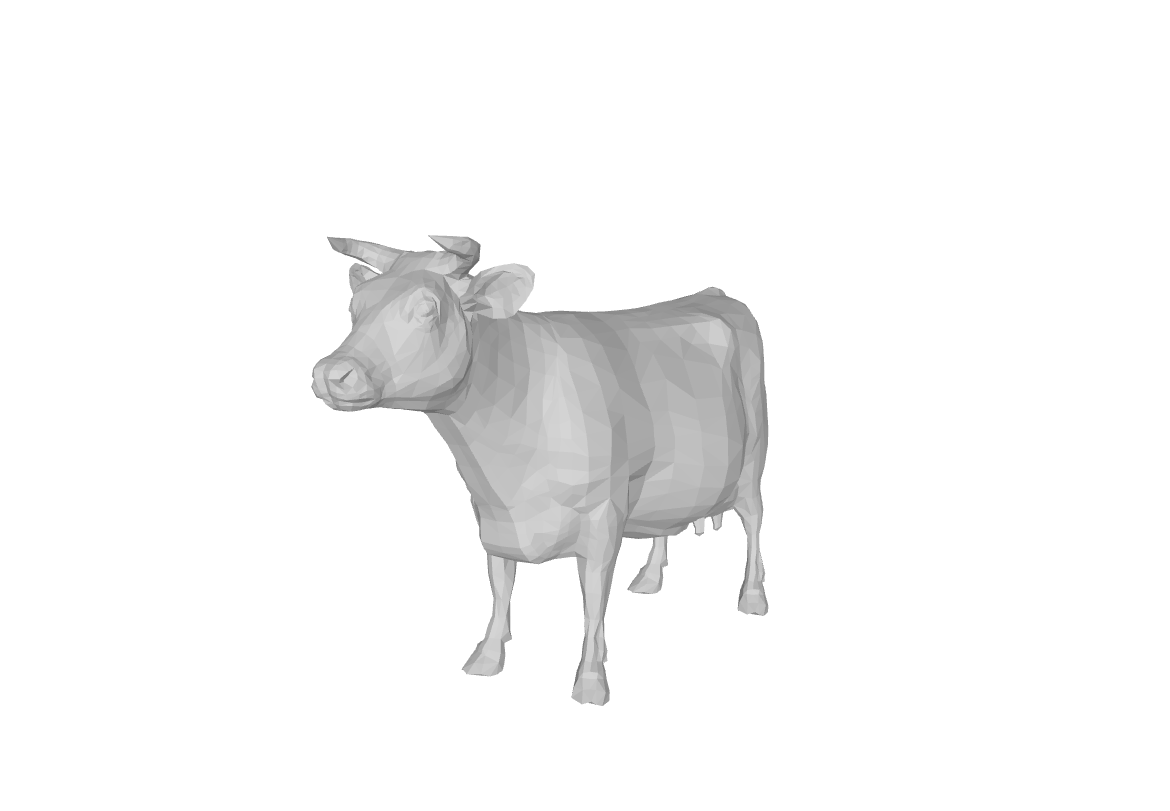
\includegraphics[width=\textwidth]{figures/cow-input.png}
                \end{center}
                \caption{Input Kasus Uji \textit{cow}}
            \end{figure}
        \item Output:
            \begin{enumerate}
                \item \texttt{maxDepth} = 3 \\
                    \begin{figure}[H]
                        \begin{center}
                            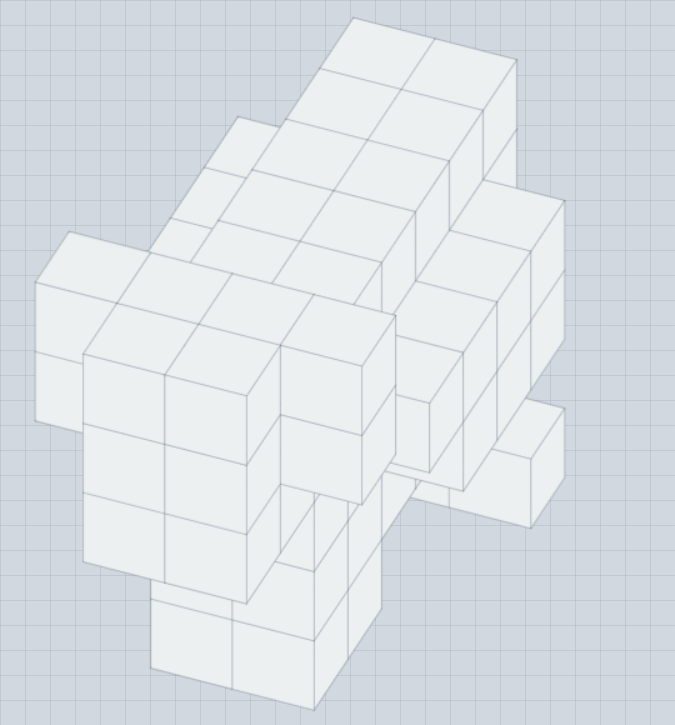
\includegraphics[width=0.3\textwidth]{figures/cow-output-3.png}
                        \end{center}
                        \caption{Hasil Kasus Uji \textit{cow} dengan \texttt{maxDepth} = 3}
                    \end{figure}
                \item \texttt{maxDepth} = 5 \\
                    \begin{figure}[H]
                        \begin{center}
                            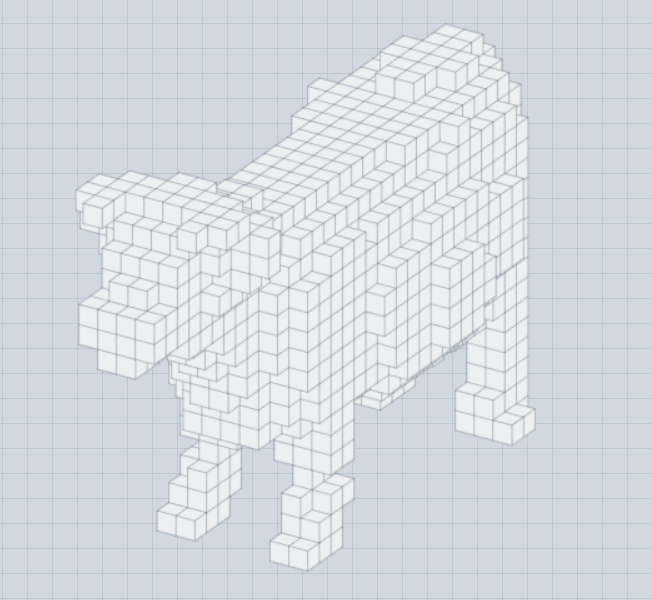
\includegraphics[width=0.3\textwidth]{figures/cow-output-5.png}
                        \end{center}
                        \caption{Hasil Kasus Uji \textit{cow} dengan \texttt{maxDepth} = 5}
                    \end{figure}
                \item \texttt{maxDepth} = 7 \\
                    \begin{figure}[H]
                        \begin{center}
                            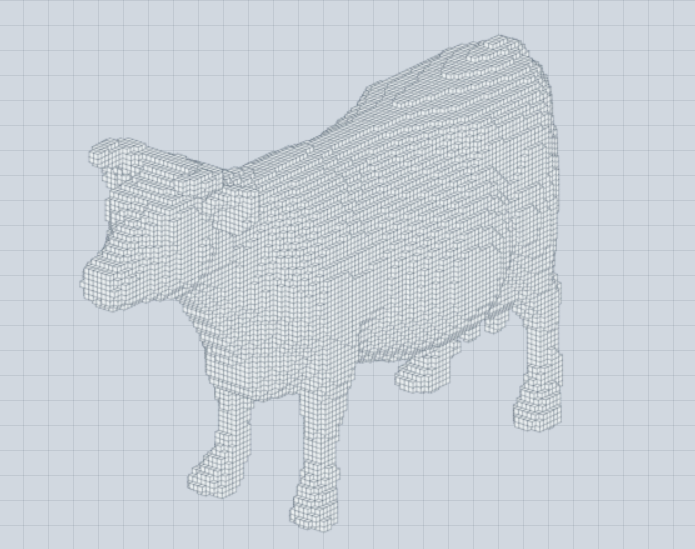
\includegraphics[width=0.3\textwidth]{figures/cow-output-7.png}
                        \end{center}
                        \caption{Hasil Kasus Uji \textit{cow} dengan \texttt{maxDepth} = 7}
                    \end{figure}
            \end{enumerate}
    \end{itemize}
    
    \subsection{Kasus Uji Objek \textit{teapot}}\label{sub:Kasus Uji Objek \textit{teapot}} % (fold)
    \begin{itemize}
        \item Input :
            \begin{figure}[H]
                \begin{center}
                    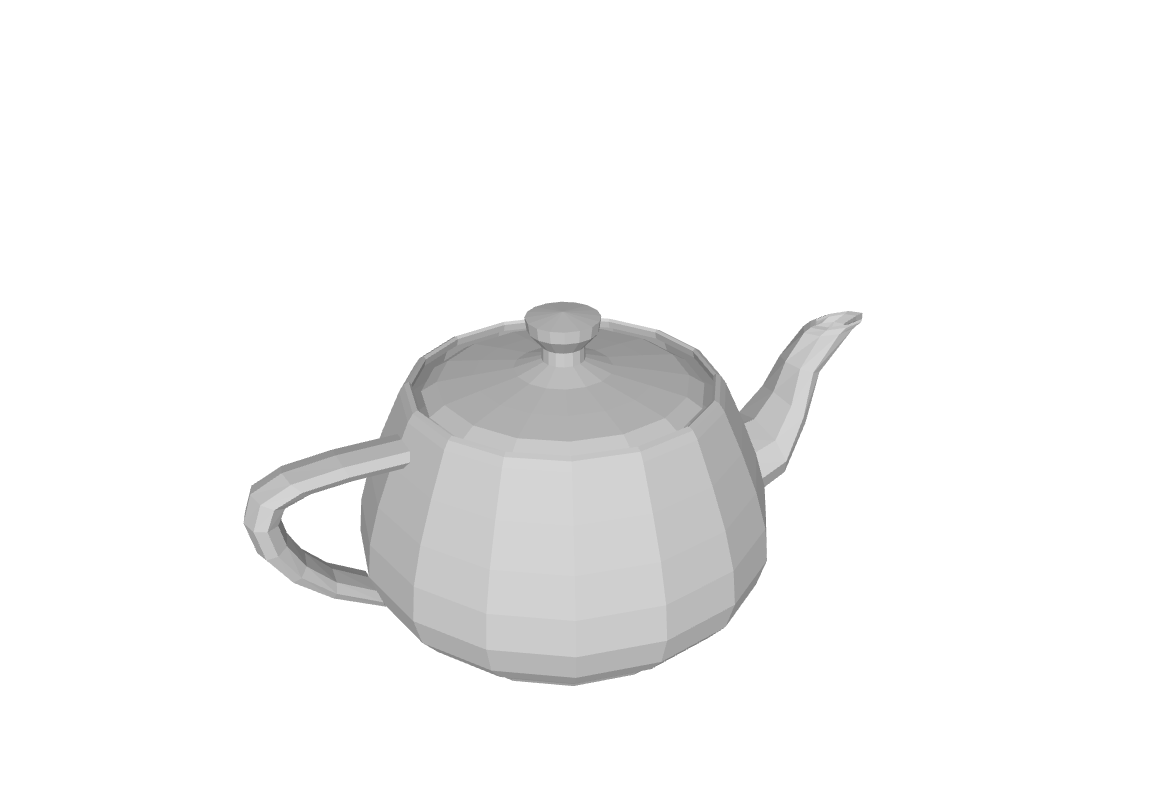
\includegraphics[width=\textwidth]{figures/teapot-input.png}
                \end{center}
                \caption{Input Kasus Uji \textit{teapot}}
            \end{figure}
        \item Output:
            \begin{enumerate}
                \item \texttt{maxDepth} = 3 \\
                    \begin{figure}[H]
                        \begin{center}
                            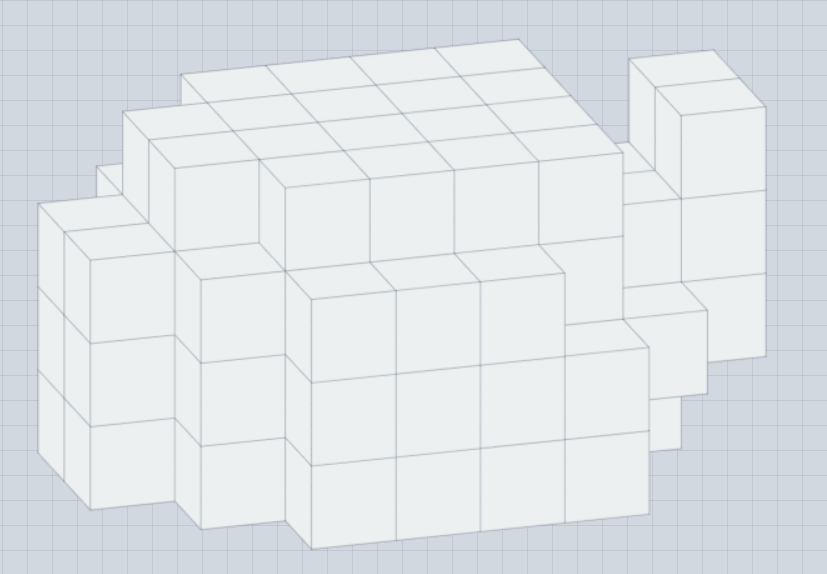
\includegraphics[width=0.3\textwidth]{figures/teapot-output-3.png}
                        \end{center}
                        \caption{Hasil Kasus Uji \textit{teapot} dengan \texttt{maxDepth} = 3}
                    \end{figure}
                \item \texttt{maxDepth} = 5 \\
                    \begin{figure}[H]
                        \begin{center}
                            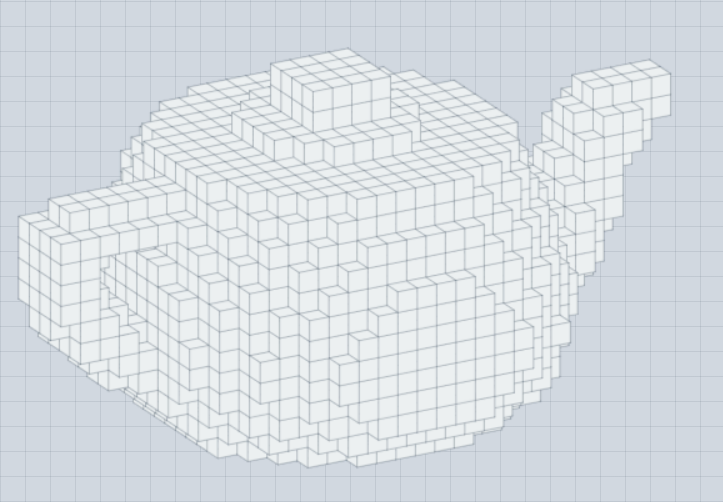
\includegraphics[width=0.3\textwidth]{figures/teapot-output-5.png}
                        \end{center}
                        \caption{Hasil Kasus Uji \textit{teapot} dengan \texttt{maxDepth} = 5}
                    \end{figure}
                \item \texttt{maxDepth} = 7 \\
                    \begin{figure}[H]
                        \begin{center}
                            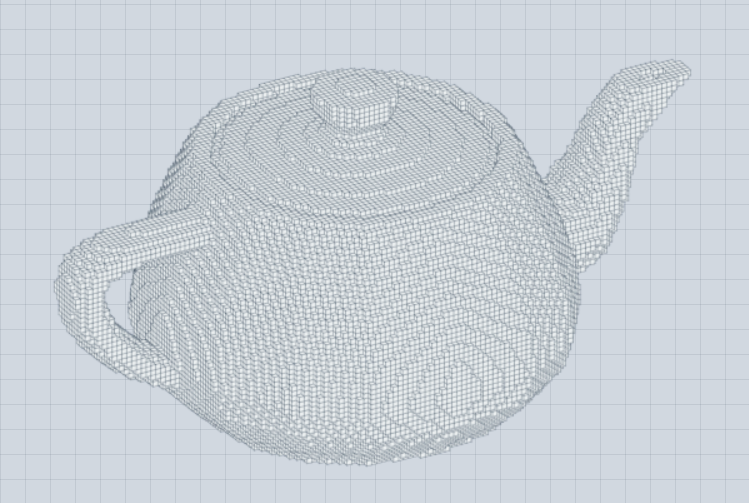
\includegraphics[width=0.3\textwidth]{figures/teapot-output-7.png}
                        \end{center}
                        \caption{Hasil Kasus Uji \textit{teapot} dengan \texttt{maxDepth} = 7}
                    \end{figure}
            \end{enumerate}
    \end{itemize}

\subsection{Hasil Pengujian}\label{sub:Hasil Pengujian} % (fold)
Berikut adalah ringkasan hasil pengujian kasus uji yang sudah
dilakukan beserta jumlah \textit{voxel}, \textit{vertex}, dan \textit{faces} yang terbentuk.
\begin{table}[!htbp]
    \begin{center}
        \begin{tabular}[\textwidth]{|c|L{4cm}|c|c|c|}
            \hline
            \textbf{No} & \textbf{Deskripsi Kasus} & \textbf{Voxel} &
            \textbf{Vertex} & \textbf{Faces} \\
            \hline
            1 & \textit{cow} \texttt{maxDepth} = 3 & 88 & 704 & 528 \\
            \hline
            2 & \textit{cow} \texttt{maxDepth} = 5 & 1362 & 10896 & 8172 \\
            \hline
            3 & \textit{cow} \texttt{maxDepth} = 7 & 22864 & 182912 & 137184 \\
            \hline
            4 & \textit{teapot} \texttt{maxDepth} = 3 & 108 & 864 & 648 \\
            \hline
            5 & \textit{teapot} \texttt{maxDepth} = 5 & 1748 & 13984 & 10488 \\
            \hline
            6 & \textit{teapot} \texttt{maxDepth} = 7 & 29565 & 236520 & 177390 \\
            \hline
        \end{tabular}
        \caption{Ringkasan Hasil Pengujian Kasus Uji}
    \end{center}
\end{table}

\pagebreak
% subsection Hasil Pengujian (end)
% section Pengujian (end)
